\section{動作結果}\label{sec:result}
最終的に組み立てたものが図~\ref{fig:complete}である.

\begin{figure}[htbp]
  \centering
  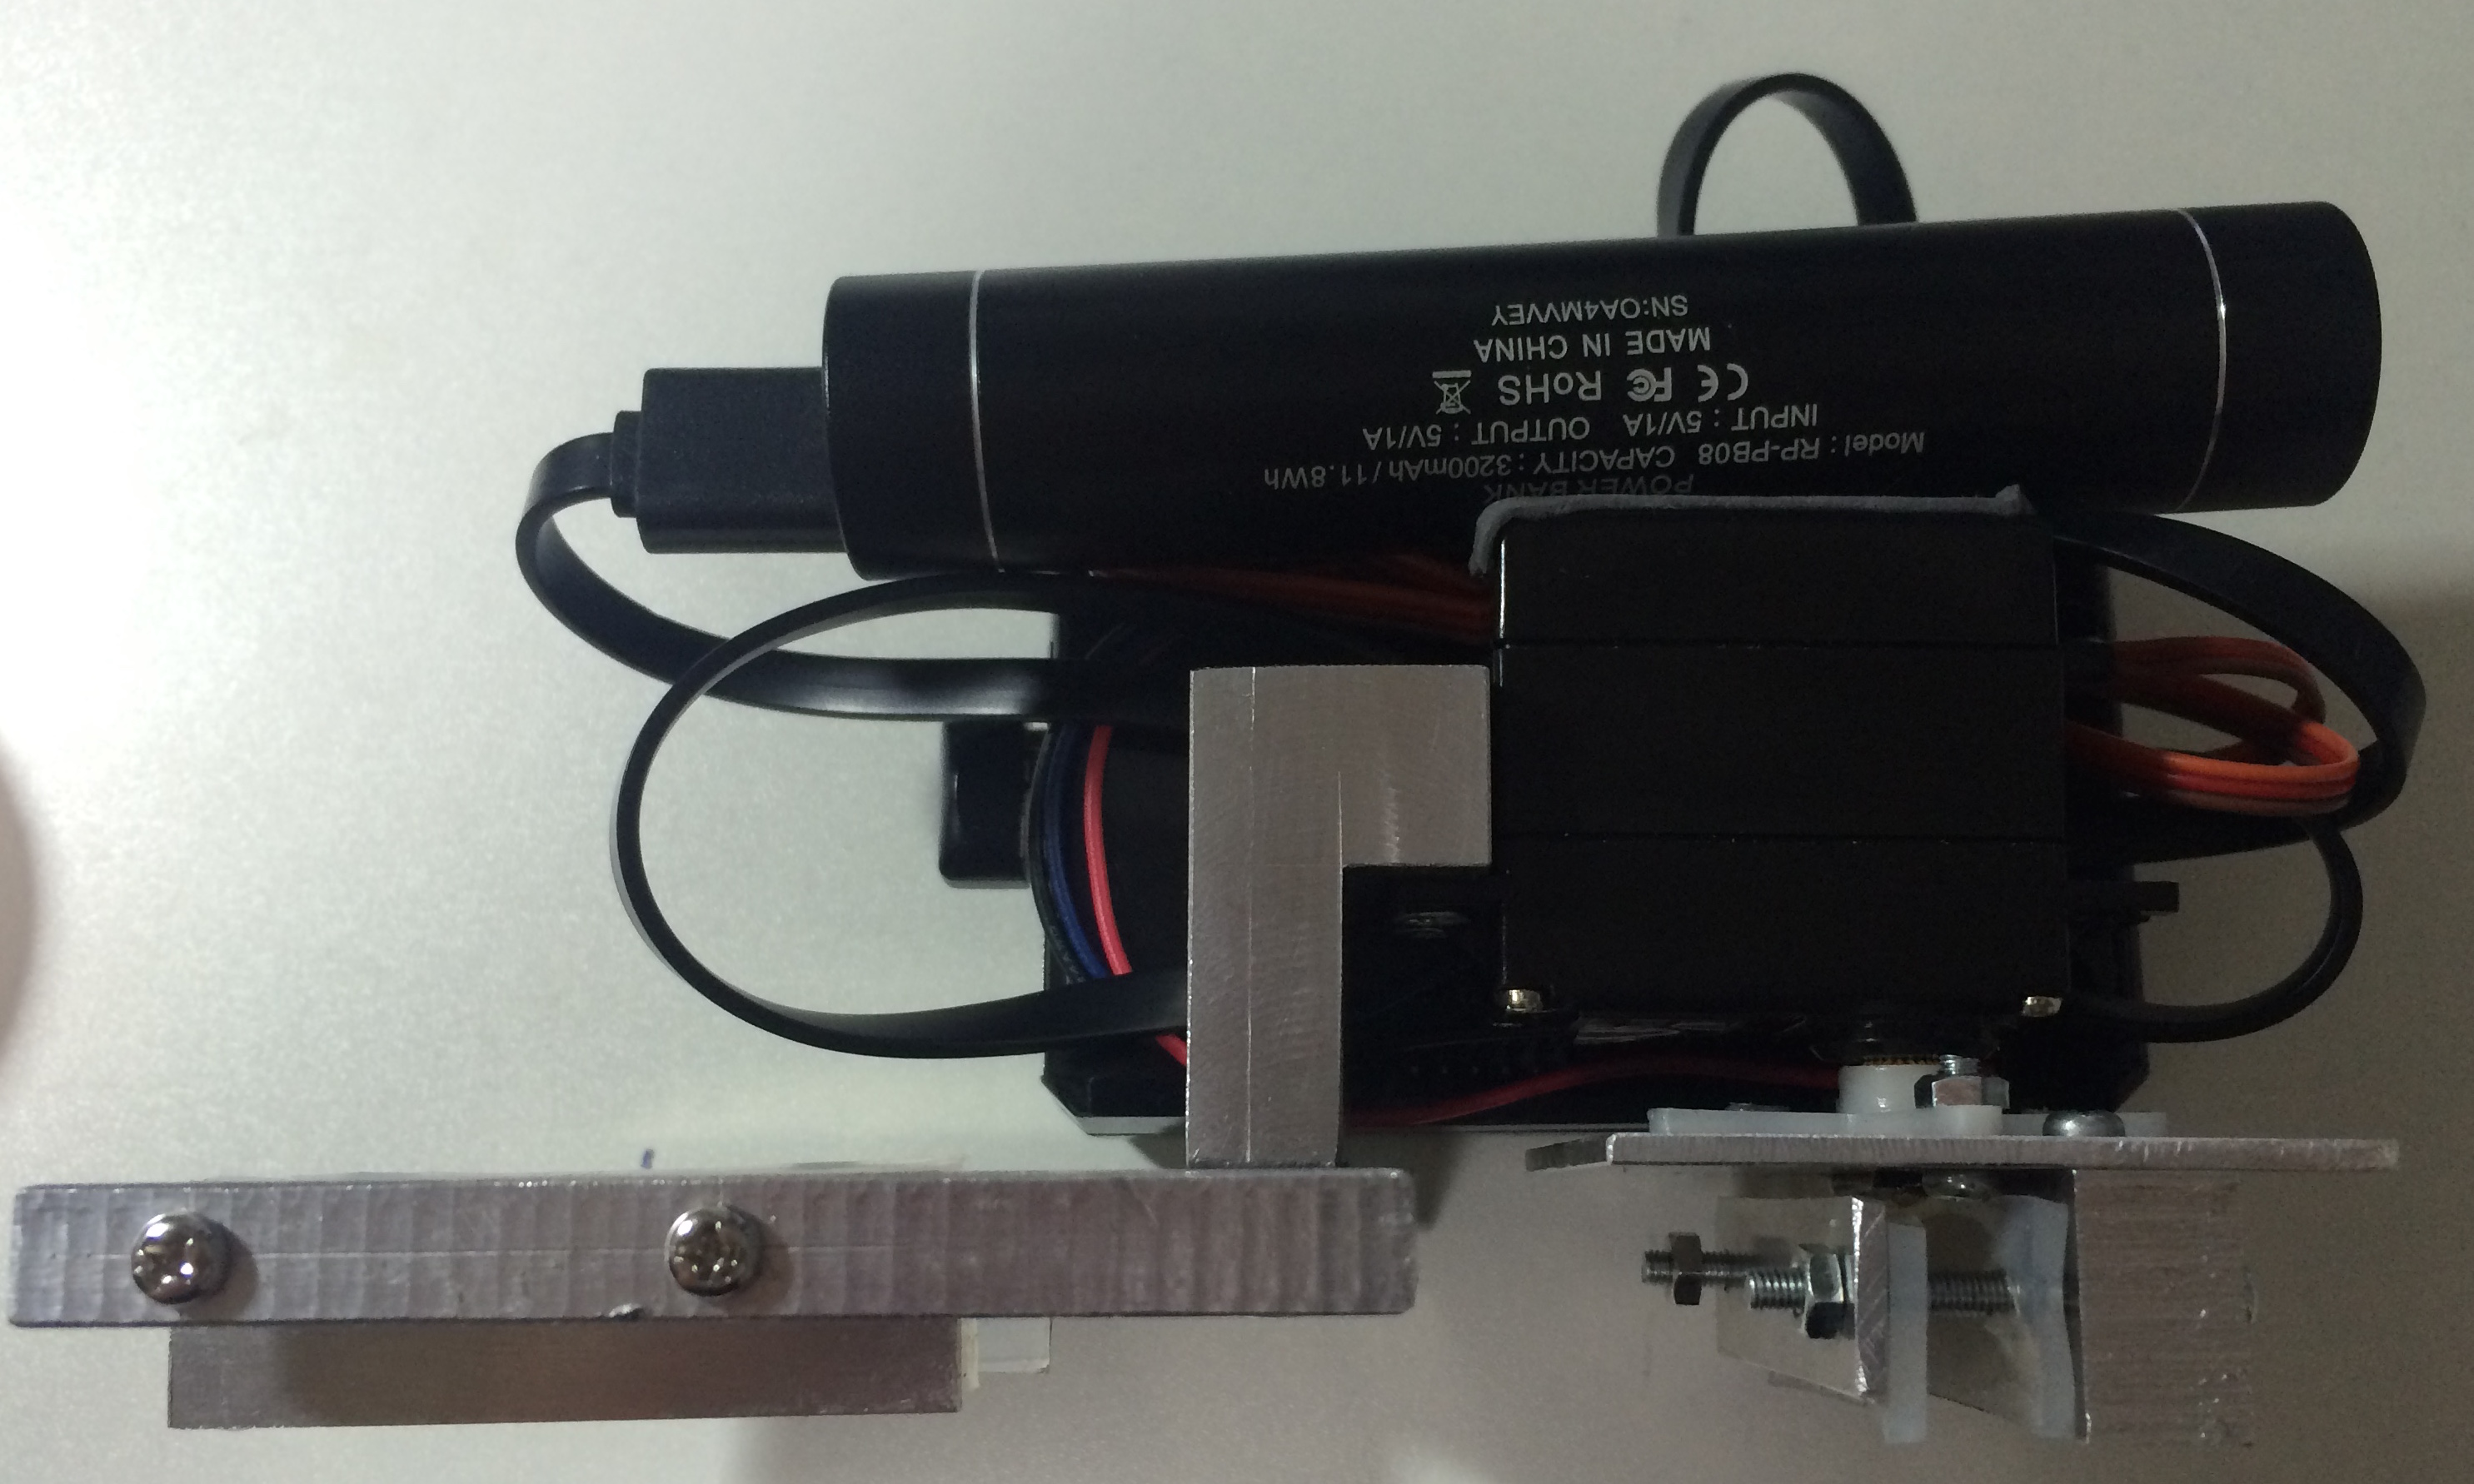
\includegraphics[width=0.35\textwidth]{./assets/complete.eps}
  \caption{ドア取り付け部分}
  \label{fig:complete}
\end{figure}

スマートフォンやPCのブラウザからアクセスし,ログイン,
アクセス権共有,ログ確認,鍵の開閉操作など問題なく動作した.

実際に取り付けを行うと,錠の中心軸とモータの軸とがずれている場合があるが,
一度回転を行うとモータのトルクによって位置調節が行われ,
二度目からは完全に軸が揃った状態になる.

電源に利用したモバイルバッテリーの連続稼働時間は24時間程度であった.

